\ifpdf
    \graphicspath{{figures/}{figures/comparisons}}
\else
    \graphicspath{{figures/}{figures/comparisons}}
\fi

\chapter{Structure From Motion with Sensor Fusion} \label{chap:structure_from_motion}
Normally 3D reconstruction does not stop on two image pair reconstruction. Having image or video sequence one can perform more accurate model reconstruction (SfM).
This chapter describes the possibility of enhancing Pose Estimation methods with additional Sensor Fusion rotation and translation calculations. All proposed and implemented algorithms were tested in terms of speed, accuracy and effectiveness in the Structure From Morion process.
\section{Concept - enhancing Pose estimation}
For any point in the image, which has a corresponding 3D point the following condition is met:
\begin{equation} \label{eq:projectionEquation}
 \textbf{x} = \textbf{P}\textbf{X}
\end{equation}
where \textbf{x} is image point expressed in homogenous coordinates (x , y , 1) and \textbf{X} homogenous 3D point (X , Y , Z , 1). The perspective projection camera matrix is as follows: 
\begin{equation} \label{eq:projectionEquation}
 P = K * \begin{bmatrix}R\mid t\end{bmatrix}
\end{equation}
where \textbf{R} is camera rotation and \textbf{t} is translation both relative to object coordinate system.
\subsection{Rotation enhancements}
Applying the similar approach as previously when enhancing epipolar equations, but this time expressing rotation as \textbf{sum} of initial rotation matrix and error matrix, it can be noted (with properties of matrix operations) that:
\begin{equation} \label{eq:projectionRotError1}
\begin{array}{rcl}
 \textbf{x} & = & \textbf{K} \begin{bmatrix}\textbf{R}_{init} + \textbf{R}_{error}\mid \textbf{t}\end{bmatrix} \textbf{X} \\
 \textbf{x} & = & \textbf{K} \begin{bmatrix}\textbf{R}_{init}\mid \textbf{0}\end{bmatrix} \textbf{X} + \textbf{K} \begin{bmatrix}\textbf{R}_{error}\mid \textbf{t}\end{bmatrix} \textbf{X} \\
 \textbf{x} - \textbf{K} \begin{bmatrix}\textbf{R}_{init}\mid \textbf{0}\end{bmatrix} & = & \textbf{K} \begin{bmatrix}\textbf{R}_{error}\mid \textbf{t}\end{bmatrix} \textbf{X}
\end{array}
\end{equation}
Substituting $\textbf{x}_{m} = \textbf{x} - \textbf{K} \begin{bmatrix}\textbf{R}_{init}\mid \textbf{0}\end{bmatrix}$ the following is received: 
\begin{equation} \label{eq:projectionRotError2}
\textbf{x}_{m} = \textbf{K}\begin{bmatrix}\textbf{R}_{error}\mid \textbf{t}\end{bmatrix}\textbf{X}
\end{equation}
This equation can be solved using a standard pose calculating algorithms and thus values of $\textbf{R}_{error}$ and \textbf{t} can be found. In other words initial rotation can be used in the pose estimation process in order to allow focus on the rotation error and translation estimation.
\subsection{Rotation \& translation enhancements}
Similar to equation \ref{eq:projectionRotError1}, if translation \textbf{t} is expressed as sum of $\textbf{t}_{init}$ and $\textbf{t}_{error}$ :
\begin{equation} \label{eq:projectionRotError3}
\begin{array}{rcl}
 \textbf{x} & = & \textbf{K} \begin{bmatrix}\textbf{R}_{init} + \textbf{R}_{error}\mid \textbf{t}_{init} + \textbf{t}_{error}\end{bmatrix} \textbf{X} \\
 \textbf{x} & = & \textbf{K} \begin{bmatrix}\textbf{R}_{init}\mid \textbf{t}_{init}\end{bmatrix} \textbf{X} + \textbf{K} \begin{bmatrix}\textbf{R}_{error}\mid \textbf{t}_{error}\end{bmatrix} \textbf{X} \\
 \textbf{x} - \textbf{K} \begin{bmatrix}\textbf{R}_{init}\mid \textbf{T}_{init}\end{bmatrix} & = & \textbf{K} \begin{bmatrix}\textbf{R}_{error}\mid \textbf{t}_{error}\end{bmatrix} \textbf{X}
\end{array}
\end{equation}
end in the end by substituting $\textbf{x}_{n} = \textbf{x} - \textbf{K} \begin{bmatrix}\textbf{R}_{init}\mid \textbf{T}_{init}\end{bmatrix}$ the following is received: 
\begin{equation} \label{eq:projectionRotError4}
\textbf{x}_{n} = \textbf{K} \begin{bmatrix}\textbf{R}_{error}\mid \textbf{t}_{error}\end{bmatrix} \textbf{X}
\end{equation}
This equation can also be solved using a standard pose calculating algorithms (\cite{website:poseEstimation}) and thus values of $\textbf{R}_{error}$ and $\textbf{t}_{error}$ can be found. In other words initial rotation and translation can be used in the pose estimation process in order to allow focus on the rotation error and translation error estimation.
\section{General implementation aspects}
OpenCV already has the rotation and translation enhanced pose estimation implemented. The initial rotation and translation can be passed as input variables. Pose estimation method wrappers implementations are as follows: 
\begin{lstlisting}
Mutiview::FindPoseEstimation(
        cv::Mat &rvec,
        cv::Mat &t,
        cv::Mat &R,
        cv::Mat &K,
        cv::Mat &distCoeffs,
        std::vector<cv::Point3d> ppcloud,
        std::vector<cv::Point2d> imgPoints,
        vector<int> inliers) 
Mutiview::FindPoseEstimationEnhanced(
        cv::Mat &rvec,
        cv::Mat &t,
        cv::Mat &R,
        cv::Mat &RInit,
        cv::Mat &TInit,
        cv::Mat &K,
        cv::Mat &distCoeffs,
        std::vector<cv::Point3d> ppcloud,
        std::vector<cv::Point2d> imgPoints,
        vector<int> inliers)
\end{lstlisting}
and their detailed implementations can be found in 'Mutiview.cpp' file.

\subsection{Reconstruction process strategy}
Finally, all methods described in this thesis can be combined in different reconstruction strategies. For the initialisation of 3D cloud point the following strategies can be used:
\begin{enumerate} 
\item \textbf{Known rotations and translations}, which theoretically allows for an metrical reconstruction
\item \textbf{Known rotations}, where translation is estimated with an alternative 3-point algorithm
\item \textbf{Noisy rotations}, where enhanced 8-point fundamental or 5-point essential algorithms are used in order to calculate rotation error and relative translation 
\item \textbf{Unknown external camera parameters}, where standard 8-point fundamental or 5-point essential algorithms are used in order to calculate rotation and relative translation
\end{enumerate}
For the pose estimation the following methodologies can be used:
\begin{enumerate}
\item \textbf{Known rotations and translations}, where no additional calculations are required and an metrical model can be acquired
\item \textbf{Initial rotation}, where relative translation needs to be calculated
\item \textbf{Noisy rotation and translation}, where both rotation and translation errors need to be calculated
\item \textbf{Unknown external camera parameters}, where standard pose estimation has to be used
\end{enumerate}
All proposed strategies can be chosen in desktop application.
% ----------------------- contents from here ------------------------
\section{Evaluation}
As regards the speed test, it included the measurement of the reconstruction execution time. In the accuracy testing Sampson Error measurement was used (Section 12.4 of \cite{HartleyMultipleView}). This variable measures the distance between all points and their corresponding epipolar lines in an image. The smaller this value is, the better precision of \textbf{F} was achieved during epipolar equation resolving. This also can be defined from other perspective - the more accurate \textbf{R} and \textbf{T} are estimated, the smaller Sampson value will be. Effectiveness was tested by visual comparison of reconstructed 3D cloud points. Basically author checked if these spatially reconstructed models has the same contours as photographed objects.

\subsection{Acquiring datasets}
For the purpose of evaluation the following datasets were captured with the implemented ''Sensor Enhanced Images Camera'' application and Nexus 5 camera:
\begin{enumerate} 
\item Warsaw University of technology main building
\item Advertisement Pole 
\item Warsaw Business School Gate and Entrance
\item Warsaw Shopping Center Back
\item Warsaw Shopping Center Front
\end{enumerate}
All of these datasets can be found on attached CD. \\ 
Since most of the algorithms proposed in the Chapter 4 require internal camera parameters to be known, the camera used in the course of conducting this study was calibrated and its internal camera parameters were stored in \textit{''outcameradata.yml''} file using OpenCV calibration sample code. 
\subsection{Test Environment}
All tests were performed on MacBook Air with 1.7GHz dual-core Intel Core i7 processor and 8GB 1600MHz DDR3 RAM using ''Enhanced 3D Reconstructer'' implemented as described in the Implementation chapter. Epipolar lines accuracy calculation tests which allowed for measuring total Sampson errors and execution time were run on the ''Warsaw University of Technology'' dataset. Finally, for each dataset the most effective methods were used to reconstruct sparse 3D models. 
\subsection{Testing initial pair reconstruction methods} \label{sec:Testin2Views}
The key question to be answered at this point was whether the proposed sensor enhancement gave better results than the standard algorithms.
The following methods were tested:
\begin{enumerate}
\item \textbf{Standard 8-point} - based on the 8-point fundamental matrix decomposition, implemented in OpenCV
\item \textbf{Enhanced 8-point} - the proposed camera rotation enhanced version of the above 8-point algorithm
\item \textbf{Alternative 3-point} - the proposed 3-point algorithm for translation estimation.
\item \textbf{Known rotations and translations} - calculation from known cameras rotations and translations
\item \textbf{Standard essential 5-point} - based on the 5-point essential matrix decomposition, implemented in \cite{website:relativePoseLibrary}
\item \textbf{Enhanced essential 5-point} - similar to 2. rotation-enhanced version of the above 5-point algorithm
\end{enumerate}
\subsubsection{Accuracy - Epipolar lines correspondence}
In the case of initial pair images one of the most important factors include the epipolar constraint. With the use of a properly estimated fundamental matrix, drawing corresponding epipolar lines in both images is possible. Furthermore, points lying on two matching epipolars lines in different images can be easily matched. In other words, epipolar lines cross exactly the same points in both images. The more accurate they are the more corresponding pairs can be found, e.g. for the purposes of performing dense reconstruction. Sampson Error is one of the metrics that can be used in order to estimate the accuracy of epipolars lines; the smaller the error's value the more accurate the lines. Its primary function is to measure the total distance between all points and their corresponding epipolar lines.\\
\begin{figure}[b!]
  \begin{center}
    \begin{tikzpicture}
      \begin{axis}[
          width=\linewidth, % Scale the plot to \linewidth
          grid=major, % Display a grid
          grid style={dashed,gray!30}, % Set the style
          xtick = {100,500,1000,5000},
          xlabel=Sift features number, % Set the labels
          xmode=log,
          log ticks with fixed point,
          ymode=log,
          log ticks with fixed point,
          ylabel=Total Sampson Error(pixels),
          legend style={at={(0.5,-0.05)},anchor=north,cells={anchor=west}}, % Put the legend below the plot
        ]
        \addplot[mark=*,blue] table[x=Number of Sift features,y=8-point OpenCV,col sep=comma] {SampsonTotal.csv}; 
        \addplot[mark=*,red] table[x=Number of Sift features,y=8-point enhanced,col sep=comma] {SampsonTotal.csv};
        \addplot[mark=*,orange] table[x=Number of Sift features,y=Alternative 3-point,col sep=comma] {SampsonTotal.csv}; 
        \addplot[mark=*,pink] table[x=Number of Sift features,y=Known rot and trans,col sep=comma] {SampsonTotal.csv};
        \addplot[mark=*,green] table[x=Number of Sift features,y=Essential 5-point,col sep=comma] {SampsonTotal.csv};
        \addplot[mark=*,yellow] table[x=Number of Sift features,y=5-point enhanced,col sep=comma] {SampsonTotal.csv};
        \legend{Standard 8-point,Enhanced 8-point,Alternative 3-point,Known rotations and translations,Standard essential 5-point,Enhanced essential 5-point}
      \end{axis}
    \end{tikzpicture}
    \caption[Sum of Sampson Error depending on evaluated method]{Chart showing the sum of Sampson Errors in a Warsaw Universiy pictures(1024x768pixels) per various initial SIFT features sets sizes}
    \label{plot:TotalSampsonError}
  \end{center}
\end{figure}
The chart \ref{plot:TotalSampsonError} shows the total Sampson Errors for different numbers of initial SIFT features. As could have been expected the only one that is not much efficient in this regard is the \textbf{method} involving drawing epipolar lines from heuristically estimated translation and sensor fusion rotation, which produces significantly larger error than the other algorithms. \\
Each of the proposed methods could have removed different outliers during RANSAC filtering in epipolar geometry solving, therefore in order to better compare their efficiency, the average of Samson Error per a corresponding pair was calculated.
\begin{figure}[hb!]
  \begin{center}
    \begin{tikzpicture}
      \begin{axis}[
          width=\linewidth, % Scale the plot to \linewidth
          grid=major, % Display a grid
          grid style={dashed,gray!30}, % Set the style
          xtick = {100,500,1000,5000},
          xlabel=Sift features number, % Set the labels
          xmode=log,
          log ticks with fixed point,
          ymode=log,
          log ticks with fixed point,
          ylabel=Total Sampson Error per point(pixels),
          legend style={at={(0.5,-0.05)},anchor=north,cells={anchor=west}}, % Put the legend below the plot
        ]
        \addplot[mark=*,blue] table[x=Number of Sift features,y=8-point OpenCV,col sep=comma] {SampsonPerPoint.csv}; 
        \addplot[mark=*,red] table[x=Number of Sift features,y=8-point enhanced,col sep=comma] {SampsonPerPoint.csv};
        \addplot[mark=*,orange] table[x=Number of Sift features,y=Alternative 3-point,col sep=comma] {SampsonPerPoint.csv}; 
        \addplot[mark=*,pink] table[x=Number of Sift features,y=Known rot and trans,col sep=comma] {SampsonPerPoint.csv};
        \addplot[mark=*,green] table[x=Number of Sift features,y=Essential 5-point,col sep=comma] {SampsonPerPoint.csv};
        \addplot[mark=*,yellow] table[x=Number of Sift features,y=5-point enhanced,col sep=comma] {SampsonPerPoint.csv};
        \legend{Standard 8-point,Enhanced 8-point,Alternative 3-point,Known rotations and translations,Standard essential 5-point,Enhanced essential 5-point}
      \end{axis}
    \end{tikzpicture}
    \caption[Sampson Error per corresponding point depending on evaluated method]{Chart showing per point Sampson Error in a Warsaw University pictures(1024x768pixels) per various initial SIFT features sets sizes}
    \label{plot:SampsonErrorPerPoint}
  \end{center}
\end{figure}
Analysing the per pair Sampson Error results \ref{plot:SampsonErrorPerPoint} it can be noted that the proposed sensor enhanced methods did not improve accuracy of epipolar lines calculation. To present the discussed errors, estimated epipolar lines for 300 initial SIFT features set were drawn on the Figures \ref{fig:SummaryEpiLines1300} - \ref{fig:SummaryEpiLines2300}.
\begin{figure}[b!]
    \centering
    \includegraphics[width=0.8\textwidth]{summary1Sift300}
    \caption[The results of drawing estimated epipolar lines for the Warsaw University Dataset with 300 SIFT points (1st group)]{The results of drawing estimated epipolar lines for the Warsaw University Dataset with 300 SIFT points. 1) Standard Fundamental 8-point algorithm (upper pair), 2) Rotation Enhanced Fundamental 8-point algorithm (middle pair), 3) Alternative 3-point algorithm (bottom pair) }
    \label{fig:SummaryEpiLines1300}
\end{figure}
\begin{figure}[ht!]
    \centering
    \includegraphics[width=0.8\textwidth]{summary2Sift300}
    \caption[The results of drawing estimated epipolar lines for the Warsaw University Dataset with 300 SIFT points (2nd group)]{The results of drawing estimated epipolar lines for the Warsaw University Dataset with 300 SIFT points. 1) Fundamental matrix created from rotation and translation (upper pair), 2) Standard Essential matrix 5-point algorithm (middle pair), 3) Rotation Enhanced Essential 5-point algorithm (bottom pair) }
    \label{fig:SummaryEpiLines2300}
\end{figure}
It can be seen that both the standard 8-point algorithm and the proposed rotation-enhanced version return very good results in terms of epipolar lines accuracy. The alternative 3-point algorithm gives slightly worse results due to the uncompensated mobile sensors' rotation estimation error. \newline
To verify whether the epipolar lines calculation is influenced by the number of SIFT features, the same process was applied to 1000 SIFT features set (Figures \ref{fig:SummaryEpiLines11000} - \ref{fig:SummaryEpiLines21000}). 
\begin{figure}[b!]
    \centering
    \includegraphics[width=0.8\textwidth]{summary1Sift1000}
    \caption[The results of drawing estimated epipolar lines for the Warsaw University Dataset with 1000 SIFT points (1st group)]{The results of drawing estimated epipolar lines for the Warsaw University Dataset with 1000 SIFT points. 1) Standard Fundamental 8-point algorithm (upper pair), 2) Rotation Enhanced Fundamental 8-point algorithm (middle pair), 3) Alternative 3-point algorithm (bottom pair) }
    \label{fig:SummaryEpiLines11000}
\end{figure}
\begin{figure}[ht!]
    \centering
    \includegraphics[width=0.8\textwidth]{summary2Sift1000}
    \caption[The results of drawing estimated epipolar lines for the Warsaw University Dataset with 1000 SIFT points (2nd group)]{The results of drawing estimated epipolar lines for the Warsaw University Dataset with 1000 SIFT points. 1) Fundamental matrix created from rotation and translation (upper pair), 2) Standard Essential matrix 5-point algorithm (middle pair), 3)Rotation Enhanced Essential 5-point algorithm (bottom pair) }
    \label{fig:SummaryEpiLines21000}
\end{figure}
In general, the proposed enhanced algorithms are not better than standard versions in terms of accuracy of epipolar lines estimation. Epipolar lines calculated from Sensor Fusion rotation and translation do not cross corresponding points position, but the same was already shown in \ref{chap:recon_sensors} on Test dataset.
\clearpage
\subsubsection{Time comparison}
The chart \ref{plot:ExecutionTime} below shows the averaged  execution time for 100 estimation attempts.
\begin{figure}[hb!]
  \begin{center}
    \begin{tikzpicture}
      \begin{axis}[
          width=\linewidth, % Scale the plot to \linewidth
          grid=major, % Display a grid
          grid style={dashed,gray!30}, % Set the style
          xtick = {100,500,1000,5000},
          xlabel=Sift features number, % Set the labels
          xmode=log,
          log ticks with fixed point,
          ymode=log,
          ylabel=Execution time(ms),
          legend style={at={(0.5,-0.05)},anchor=north,cells={anchor=west}}, % Put the legend below the plot
        ]
        \addplot[mark=*,blue] table[x=Number of Sift features,y=8-point OpenCV,col sep=comma] {ExecutionTime.csv}; 
        \addplot[mark=*,red] table[x=Number of Sift features,y=8-point enhanced,col sep=comma] {ExecutionTime.csv};
        \addplot[mark=*,orange] table[x=Number of Sift features,y=Alternative 3-point,col sep=comma] {ExecutionTime.csv}; 
        \addplot[mark=*,pink] table[x=Number of Sift features,y=Known rot and trans,col sep=comma] {ExecutionTime.csv};
        \addplot[mark=*,green] table[x=Number of Sift features,y=Essential 5-point,col sep=comma] {ExecutionTime.csv};
        \addplot[mark=*,yellow] table[x=Number of Sift features,y=5-point enhanced,col sep=comma] {ExecutionTime.csv};
        \legend{Standard 8-point algorithm,Enhanced 8-point algorithm,Alternative 3-point algorithm,Known rotations and translations,Standard essential 5-point algorithm,Enhanced essential 5-point algorithm}
      \end{axis}
    \end{tikzpicture}
    \caption[Execution time of the proposed algorithms depending on initial SIFT feature set size]{Execution time of the proposed algorithms(1024x768pixels) per initial SIFT feature set size in Warsaw University dataset}
    \label{plot:ExecutionTime}
  \end{center}
\end{figure}
Execution time of the 8-point algorithms are very similar, which is understandable, since their implementation is nearly identical and they differ only in the characteristics of points conditioning. It can be seen, however, that execution time values of the 5-point epipolar estimations differ significantly depending on the version. In this situation probably implementation of these methods is significantly different in terms of memory allocation from OpenCV 8-point implementation. Execution time of the 3-point algorithm is few times faster than the one of the 8-point algorithms. The reconstruction with the sole use of the rotations and translations calculated from Sensor Fusion has a hundred times shorter execution time than the standard algorithms, but at the same time it does not produce properly correlated epipolar lines. It is understandable, because none epipolar geometric equation (highly resources demanding matrix problem) is resolved. 

\subsection{Testing reconstruction strategies}
As was shown to this point not every initial reconstruction method gives good results. Only the most effective techniques were used to test a few of completely different strategies for model reconstruction:
\begin{enumerate}
\item \textnormal{Standard 8-point + OpenCV Pose Estimation} 
\item \textnormal{Enhanced 8-point + OpenCV Pose Estimation} 
\item \textnormal{Enhanced 8-point + Initial Rotation and Translation OpenCV Pose Estimation} 
\item \textnormal{Alternative 3-point + OpenCV Pose Estimation}
\item \textnormal{Alternative 3-point + Initial Rotation and Translation OpenCV Pose Estimation}
%\item \textnormal{Known rotations and translations} 
\end{enumerate}
The first method gives the basic reference to standard 3D reconstruction strategy. The second one was chosen because it gave the best rotation angles estimation. Also it helps to resolve ambiguity in essential matrix decomposition, thus is expected not to fail in that matter. The third one was prepared in order to determine how the enhanced pose estimation influences the final reconstruction outcomes, especially in comparison to 2nd strategy. The strategies number four and five were used to see if the models can be produced faster without impacting the final accuracy too heavily. Finally, the fifth method was proposed in order to verify whether the entire reconstruction process can be performed using the sensor fusion data only.
\subsubsection{Accuracy}
Accuracy of the 3D reconstruction was measured using Bundle Adjustment algorithm from SBA library\cite{website:sba}. It allows for calculating the error based on the projective constraint both before and after Bundle Adjustment. If one point is visible between multiple images its 3D position can be checked with position that would be expected from camera perspective transformation. Thanks to back propagation the difference between those positions can be used to iteratively correct calculated rotations and translations of the estimated camera positions. \\
The tests performed with different strategies  for the ''Warsaw University'' dataset are presented on \ref{plot:BAError}. As expected the enhanced initial pair reconstruction and pose estimation methods have bigger impact on Bundle Adjustment camera positions error reduction.
\begin{figure}[h!]
  \begin{center}
    \begin{tikzpicture}
      \begin{axis}[
          width=0.8\linewidth, % Scale the plot to \linewidth
          grid=major, % Display a grid
          grid style={dashed,gray!30}, % Set the style
          xtick = {1,2,3,4,5},
          xticklabels = {Std8 -point+NormalPose,Enhanced8-point+NormalPose,Enhanced8-point+EnhancedPose, Alternative3-point+NormalPose,Alternative3-point+EnhancedPose},          
          xlabel=Reconstruction strategy, % Set the labels
          log ticks with fixed point,
          ylabel=Reconstruction error(in model units),
          x tick label style={rotate=90,anchor=east},
          legend style={at={(0.5,1.05)},anchor=south,cells={anchor=west}}, % Put the legend below the plot
        ]
        \addplot[mark=*,blue] table[x=ReconMethods,y=Error before BA,col sep=comma] {BAerror2.csv}; 
        \addplot[mark=*,red] table[x=ReconMethods,y=Error after BA,col sep=comma] {BAerror2.csv};
        \legend{Reconstruction Error before Bundle Adjustment,Reconstruction Error after Bundle Adjustment}
      \end{axis}
    \end{tikzpicture}
    \caption{Influence of Bundle Adjustment on the models produced with different reconstruction strategies in Warsaw University datasets}
    \label{plot:BAError}
  \end{center}
\end{figure}
In general, Bundle Adjustment process allows to rearrange and modify 3D points positions and change external parameters of estimated cameras. However, in the case of the enhanced algorithms the estimated camera positions are already very close to their optimal orientations. This allows Bundle Adjustment method to focus mainly on 3D points modifications (Figures \ref{fig:rotation_tests_enh_01} and \ref{fig:rotation_tests_enh_02}). It can be observed that the enhanced pose estimation results in further reduction of BA error when compared to the standard strategies.
\begin{figure}[h!]
    \centering
    \includegraphics[width=\textwidth]{bundleAdjustmentComparison}
    \caption[3D point clouds before and after Bundle Adjustment for enhanced 8-point with enhanced pose estimation]{3D point clouds before Bundle Adjustment (upper) and after (bottom) for enhanced 8-point with enhanced pose estimation. Warsaw University of Technology dataset with 1000 SIFT corresponding features (left - front, right - side)}
    \label{fig:BundleAdjustmentComparison}
\end{figure}

\subsubsection{Execution time}
The figure \ref{plot:ReconstructionWithoutBA} presents the execution time without Bundle Adjustment. Comparing it to the execution times in \ref{plot:ExecutionTime} one can notice that most of the time is allocated for SIFT correspondences matching, which constitutes a bottleneck in the proposed reconstruction methodology.
\begin{figure}[h!]
  \begin{center}
    \begin{tikzpicture}
      \begin{axis}[
          width=\linewidth, % Scale the plot to \linewidth
          grid=major, % Display a grid
          grid style={dashed,gray!30}, % Set the style
          xtick = {100,500,1000,5000},
          xlabel=Sift features number, % Set the labels
          xmode=log,
          log ticks with fixed point,
          ymode=normal,
          ylabel=Execution time(ms),
          legend style={at={(0.5,-0.05)},anchor=north,cells={anchor=west}}, % Put the legend below the plot
        ]
        \addplot[mark=*,blue] table[x=Number of Sift features,y=8-pointInit+NormalPoseEstim,col sep=comma] {ReconstructTotal.csv}; 
        \addplot[mark=*,red] table[x=Number of Sift features,y=Enhanced8-point+NormalPoseEstim,col sep=comma] {ReconstructTotal.csv};
        \addplot[mark=*,orange] table[x=Number of Sift features,y=Enhanced8-point+EnhancedPoseEstim,col sep=comma] {ReconstructTotal.csv}; 
        \addplot[mark=*,pink] table[x=Number of Sift features,y=Alternative3-point+NormalPoseEstim,col sep=comma] {ReconstructTotal.csv};
        \addplot[mark=*,green] table[x=Number of Sift features,y=Alternative3-point+EnhancedPoseEstim,col sep=comma] {ReconstructTotal.csv};
%        \addplot[mark=*,yellow] table[x=Number of SIFT features,y=Known Rotations and Translations,col sep=comma] {ReconstructTotal.csv};
        \legend{Standard 8-point initialisation + Normal OpenCV Pose Estimation,Enhanced 8-point initialisation + Normal Pose Estimation,Enhanced 8-point initialisation + Enhanced Pose Estimation, Alternative 3-point initialisation + Normal Pose Estimation, Alternative 3-point initialisation + Enhanced Pose Estimation}
      \end{axis}
    \end{tikzpicture}
    \caption[Total reconstruction execution time per SIFT features set size]{Total reconstruction execution time (4 images of Warsaw University with resolution 1024x768pixels) per SIFT features set size}
    \label{plot:ReconstructionWithoutBA}
  \end{center}
\end{figure}

\subsection{Effectiveness}
The numerical measurements used do not always correspond to the proper 3D model reconstructions. The following pages present the reconstruction effects of the proposed strategies. Figure \ref{fig:uni4000Comparison} shows the reconstructed effects for different initialisation pair methods and 4000 SIFT features set. It can be observed that both standard and enhanced 8-point methods produces very good results, which differ only in terms of final reconstruction scale. Alternative 3-point algorithm produces slightly worse and distorted models due to uncompensated noise in the rotations of the camera used. A model reconstructed from the known rotations and translations is very distorted, but nonetheless still recognisable. It could prove useful should a very fast reconstruction be needed.
\newline
The matter is slightly different when 400 SIFT feature points are used. In the first case all algorithms were able to find solutions close to optimal. However, in the second attempt the triangulation test, which is used to identify proper decomposition in standard 8-point approach, failed and produced an unrecognisable model (Figure \ref{fig:FailCaseFundamental}).
\newline
It can be seen that pose estimations enhancements result primarily in the reduction of outliers (Figure \ref{fig:PoseEstimationMethodComparison}).
\newline
Figure \ref{fig:UniNone4000} shows that reconstruction from the known rotations and translations produces many outliers. More reconstructed models can be found in Additional Materials.
\begin{figure}[p]
    \centering
    \includegraphics[width=0.9\textwidth]{uni4000Comparison}
    \caption[Reconstructed models for the proposed initial reconstruction methods and 4000 SIFT features]{Reconstructed models for the proposed initial reconstruction methods and 4000 SIFT features. From upper left to bottom right: 1) standard 8-point, 2) enhanced 8-point, 3) alternative 3-point, 4) known rotations and translations, 5) standard 5-point, 6) enhanced 5-point}
    \label{fig:uni4000Comparison}
\end{figure}
\begin{figure}[t!]
    \centering
    \includegraphics[width=0.9\textwidth]{uni400Comparison}
    \caption[Reconstructed models for the proposed initial reconstruction methods and 400 SIFT features]{Reconstructed models for the proposed initial reconstruction methods and 400 SIFT features. From upper left to bottom right: 1) standard 8-point, 2) enhanced 8-point, 3) alternative 3-point, 4) known rotations and translations, 5) standard 5-point, 6) enhanced 5-point}
    \label{fig:uni400Comparison}
\end{figure}
\begin{figure}[p]
    \centering
    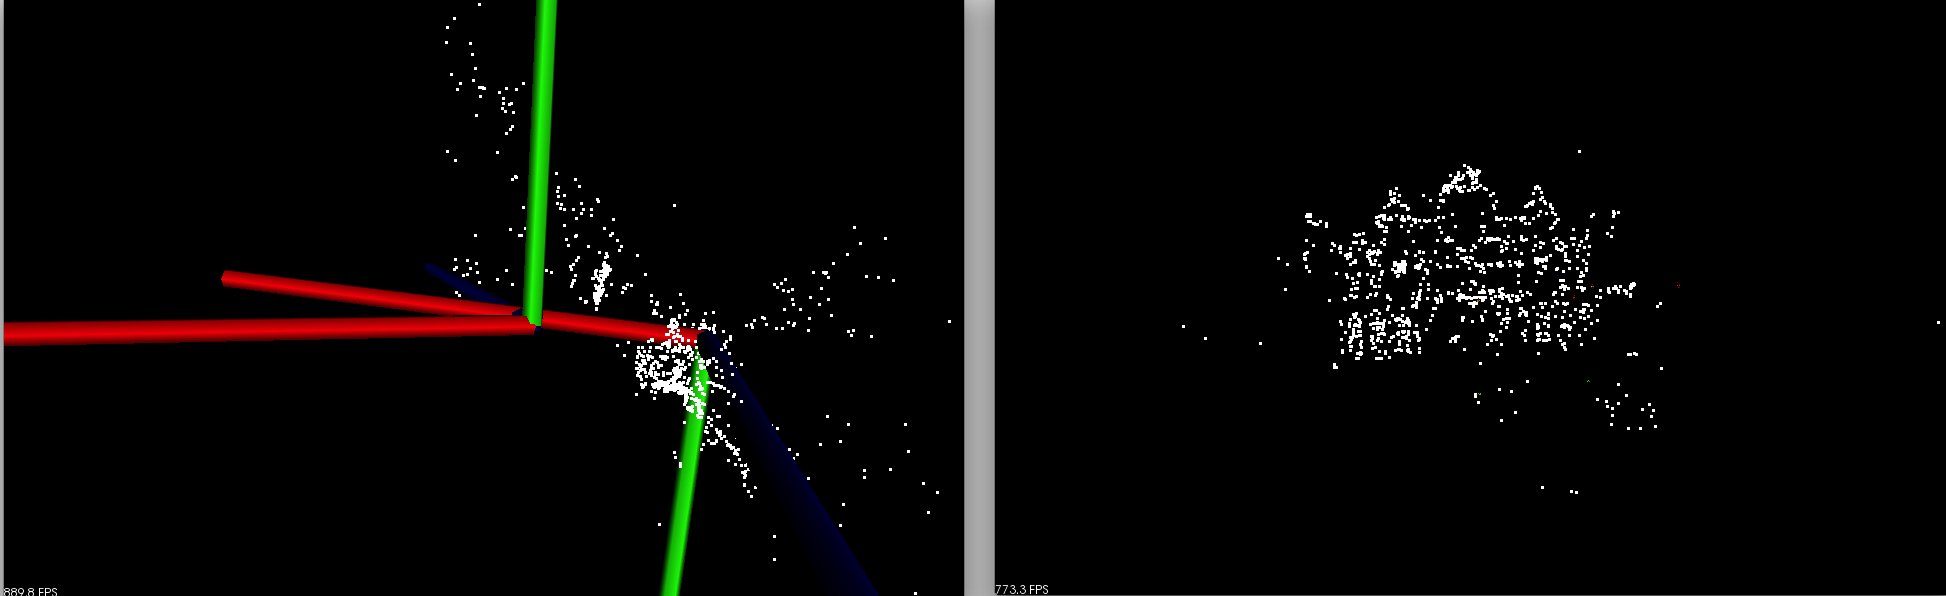
\includegraphics[width=0.9\textwidth]{FailCaseFundamental}
    \caption[Fail test case of Standard 8-point triangulation in comparison to fortunate reconstruction]{Fail test case of Standard 8-point triangulation(left) in comparison to fortunate reconstruction(right)}
    \label{fig:FailCaseFundamental}
\end{figure}
\begin{figure}[p]
    \centering
    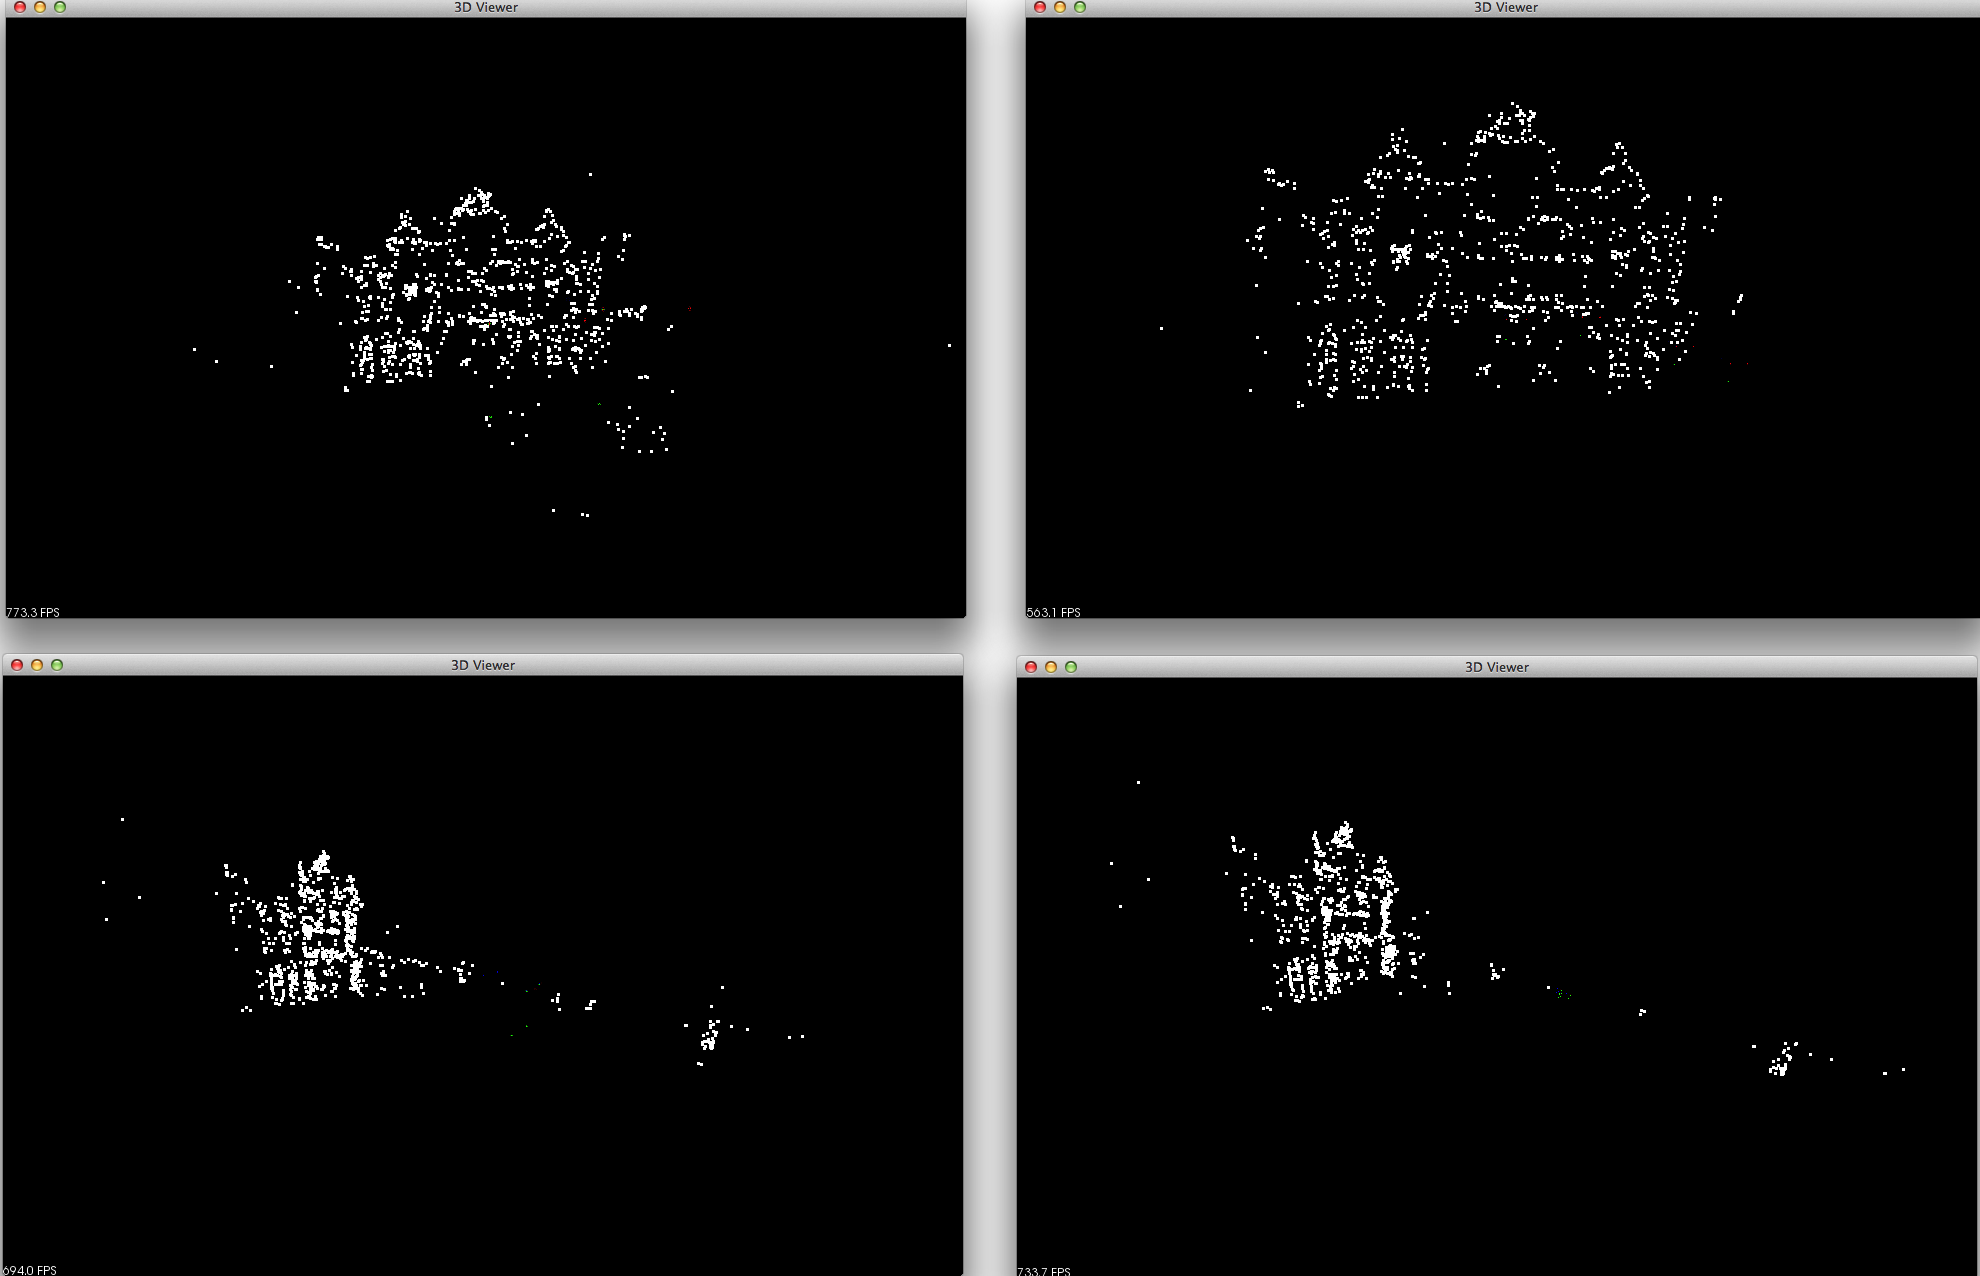
\includegraphics[width=0.9\textwidth]{PoseEstimationMethodComparison}
    \caption[Pose estimation methods comparison]{Pose estimation methods comparison (Views from front and side). Left: Normal Pose Estimation, right: Enhanced Rotation and Translation Pose Estimation. Less outliers appear in the reconstruction if enhancement is applied.}
    \label{fig:PoseEstimationMethodComparison}
\end{figure}
\begin{figure}[p]
    \centering
    \includegraphics[height=18cm]{uniNone4000}
    \caption[Reconstruction results from known translations and rotations from different angles]{Reconstruction results from known translations and rotations from different angles. The upper one shows the front face of building, the others present views from side angles. In the reconstructed model many outliers are present.}
    \label{fig:UniNone4000}
\end{figure}

% ---------------------------------------------------------------------------
% ----------------------- end of thesis sub-document ------------------------
% ---------------------------------------------------------------------------
